\section{Завдання}
\begin{enumerate}
  \item Залежно від номера прізвища за списком вибрати область індивідуального завдання. Узгодити з викладачем фрагмент програми для аналізу відповідно до індивідуального завдання.
  \item Побудувати правила граматики. Перевірити, чи не містить граматика непродуктивні та недосяжні символи.
  \item Побудувати множину ВПЕРШ та ВПІСЛЯ і, якщо необхідно, функцію СЛІД.
  \item Побудувати таблицю переходів.
  \item Побудувати керувальну таблицю.
  \item Перевірити роботу розпізнавача експериментально.
\end{enumerate}

\section{Побудова правил граматики}
\subsection{Задані ланцюжки та текст завдання}
Оператор присвоювання арифметичного виразу, до складу якого входять:
ідентифікатори, операції “+”, “-“ ,”*”,”/\/”, вкладені дужки.

\begin{enumerate}
    \item \verb|i = i + ( i - i );|
    \item \verb|i = i * ( i + ( i / i ) - i );|
    \item \verb|i = i + ( i + i );|
\end{enumerate}

\clearpage
\subsection{Опис граматики}
\begin{enumerate}
    \item  \verb|I| $\to$ \verb|i = iO(ER);|
    \item  \verb|O| $\to$ \verb|*|
    \item  \verb|O| $\to$ \verb|/|
    \item  \verb|O| $\to$ \verb|+|
    \item  \verb|O| $\to$ \verb|-|
    \item  \verb|E| $\to$ \verb|i|
    \item  \verb|E| $\to$ \verb|(iOER)|
    \item  \verb|R| $\to$ \verb|OER|
    \item  \verb|R| $\to$ \verb|$|
\end{enumerate}

\subsection{Перевірка на непродуктивність}
\begin{enumerate}
    \item  O R
    \item  O R E 
    \item  O R E I
    \item  нема непродуктивних символів
\end{enumerate}

\subsection{Перевірка на недосяжність}
\begin{enumerate}
    \item  I
    \item  I O E R
    \item  нема недосяжних символів
\end{enumerate}

\clearpage
\subsection{Перепишемо граматику додавши граматичні входження у правій частині}
\begin{enumerate}
    \item  \verb|I| $\to$ i\textsubscript{11} = i\textsubscript{13}O\textsubscript{1}(\textsubscript{15}E\textsubscript{1}R\textsubscript{1})\textsubscript{18};
    \item  \verb|O| $\to$ \verb|*|
    \item  \verb|O| $\to$ \verb|/|
    \item  \verb|O| $\to$ \verb|+|
    \item  \verb|O| $\to$ \verb|-|
    \item  \verb|E| $\to$ i\textsubscript{61}
    \item  \verb|E| $\to$ (\textsubscript{71}i\textsubscript{72}O\textsubscript{7}E\textsubscript{7}R\textsubscript{7})\textsubscript{76}
    \item  \verb|R| $\to$ O\textsubscript{8}E\textsubscript{8}R\textsubscript{8}
    \item  \verb|R| $\to$ \verb|$|
\end{enumerate}


\section{Побудова SLR(1) розпізнавача}
\subsection{Побудова функції ВПЕРШ()}
\begin{enumerate}
  \item ВПЕРШ( i\textsubscript{11} ) = \{ i\textsubscript{11} \} 
  \item ВПЕРШ( = ) = \{ = \} 
  \item ВПЕРШ( i\textsubscript{13} ) = \{ i\textsubscript{13} \} 
  \item ВПЕРШ( O\textsubscript{1} ) = \{ O\textsubscript{1}, *, /, +, - \} 
  \item ВПЕРШ( (\textsubscript{15} ) = \{ (\textsubscript{15} \} 
  \item ВПЕРШ( E\textsubscript{1} ) = \{ E\textsubscript{1}, i\textsubscript{61}, (\textsubscript{71} \} 
  \item ВПЕРШ( R\textsubscript{1} ) = \{ R\textsubscript{1}, O\textsubscript{8}, *, /, +, - \} 
  \item ВПЕРШ( )\textsubscript{18} ) = \{ )\textsubscript{18} \} 
  \item ВПЕРШ( ; ) = \{ ; \} 

  \item ВПЕРШ( * ) = \{ * \} 
  \item ВПЕРШ( / ) = \{ / \} 
  \item ВПЕРШ( + ) = \{ + \} 
  \item ВПЕРШ( - ) = \{ - \} 
  \item ВПЕРШ( i\textsubscript{61} ) = \{ i\textsubscript{61} \} 

  \item ВПЕРШ( (\textsubscript{71} ) = \{ (\textsubscript{71} \} 
  \item ВПЕРШ( i\textsubscript{72} ) = \{ i\textsubscript{72} \} 
  \item ВПЕРШ( O\textsubscript{7} ) = \{ O\textsubscript{7}, *, /, +, - \}
  \item ВПЕРШ( E\textsubscript{7} ) = \{ E\textsubscript{7}, i\textsubscript{61}, (\textsubscript{71} \} 
  \item ВПЕРШ( R\textsubscript{7} ) = \{ R\textsubscript{7}, O\textsubscript{8}, *, /, +, - \} 
  \item ВПЕРШ( )\textsubscript{76} ) = \{ )\textsubscript{76} \} 

  \item ВПЕРШ( O\textsubscript{8} ) = \{ O\textsubscript{8}, *, /, +, - \}
  \item ВПЕРШ( E\textsubscript{8} ) = \{ E\textsubscript{8}, i\textsubscript{61}, (\textsubscript{71} \} 
  \item ВПЕРШ( R\textsubscript{8} ) = \{ R\textsubscript{8}, O\textsubscript{8}, *, /, +, - \} 

  \item ВПЕРШ( I\textsubscript{0} ) = \{ i\textsubscript{11} \} 
\end{enumerate}

\subsection{Побудова функції ВПІСЛЯ()}

\begin{enumerate}
  \item ВПІСЛЯ( i\textsubscript{11} ) = \{ = \} 
  \item ВПІСЛЯ( = ) = \{ i\textsubscript{13} \}
  \item ВПІСЛЯ( i\textsubscript{13} ) = \{ O\textsubscript{1}, *, /, +, - \}
  \item ВПІСЛЯ( O\textsubscript{1} ) = \{ (\textsubscript{15} \}
  \item ВПІСЛЯ( (\textsubscript{15} ) = \{ E\textsubscript{1}, i\textsubscript{61}, (\textsubscript{71} \}  
  \item ВПІСЛЯ( E\textsubscript{1} ) = \{ R\textsubscript{1}, O\textsubscript{8}, *, /, +, - \} 
  \item ВПІСЛЯ( R\textsubscript{1} ) = \{ )\textsubscript{18} \}
  \item ВПІСЛЯ( )\textsubscript{18} ) = \{ ; \} 
  \item ВПІСЛЯ( ; ) = \{ \$ \} 

  \item ВПІСЛЯ( * ) = \{ \$ \} 
  \item ВПІСЛЯ( / ) = \{ \$ \} 
  \item ВПІСЛЯ( + ) = \{ \$ \} 
  \item ВПІСЛЯ( - ) = \{ \$ \} 
  \item ВПІСЛЯ( i\textsubscript{61} ) = \{ \$ \}  
 
  \item ВПІСЛЯ( (\textsubscript{71} ) = \{ i\textsubscript{72} \}
  \item ВПІСЛЯ( i\textsubscript{72} ) = \{ O\textsubscript{7}, *, /, +, - \} 
  \item ВПІСЛЯ( O\textsubscript{7} ) = \{ E\textsubscript{7}, i\textsubscript{61}, (\textsubscript{71} \}  
  \item ВПІСЛЯ( E\textsubscript{7} ) = \{ R\textsubscript{7}, O\textsubscript{8}, *, /, +, - \} 
  \item ВПІСЛЯ( R\textsubscript{7} ) = \{ )\textsubscript{76} \} 
  \item ВПІСЛЯ( )\textsubscript{76} ) = \{ \$ \}

  \item ВПІСЛЯ( O\textsubscript{8} ) = \{ E\textsubscript{8}, i\textsubscript{61}, (\textsubscript{71} \} 
  \item ВПІСЛЯ( E\textsubscript{8} ) = \{ R\textsubscript{8}, O\textsubscript{8}, *, /, +, - \} 
  \item ВПІСЛЯ( R\textsubscript{8} ) = \{ \$ \}

  \item ВПІСЛЯ( I\textsubscript{0} ) = \{ \$ \} 
  \item ВПІСЛЯ( h\textsubscript{0} ) = \{ I\textsubscript{0}, i\textsubscript{11} \} 
\end{enumerate}

\subsection{Побудова функції СЛІД()}
\begin{enumerate}
  \item СЛІД( I ) = \{ \$ \} 
  \item СЛІД( O ) = \{ (, i \} 
  \item СЛІД( E ) = \{ ), *, +, -, / \} 
  \item СЛІД( R ) = \{ ) \} 
\end{enumerate}

\clearpage
\subsection{Побудова таблиці переходів}
\begin{figure}[h!]
  \centering
  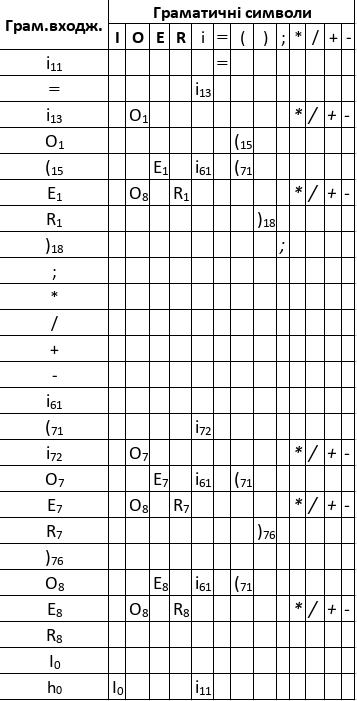
\includegraphics[width=12cm]{reports/formals/assets/go.jpeg}
\end{figure}

\clearpage
\subsection{Побудова керуючої таблиці}
\begin{figure}[h!]
  \centering
  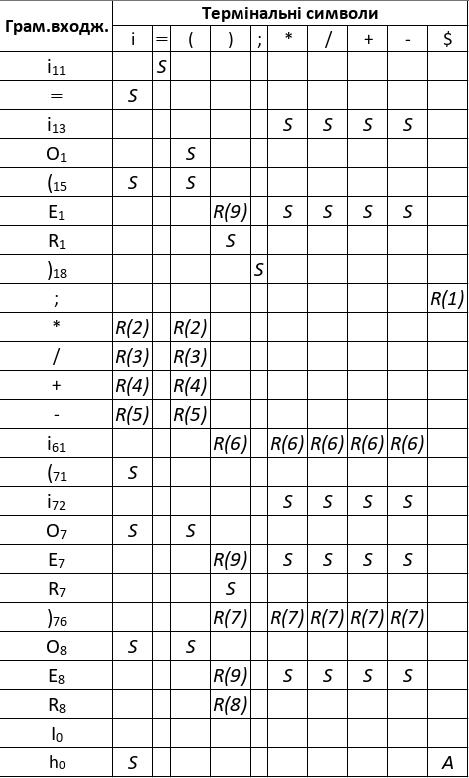
\includegraphics[width=14cm]{reports/formals/assets/action.jpeg}
\end{figure}

\clearpage
\subsection{Перевірка роботи парсеру на ланцюжках}
\textbf{PS}: не звертайте уваги на символ ` перед =, його треба було проставити щоб excel не сприймав запис як формулу.\\

Перевірка ланцюжка \verb|i = i + ( i - i );|
\begin{figure}[h!]
  \centering
  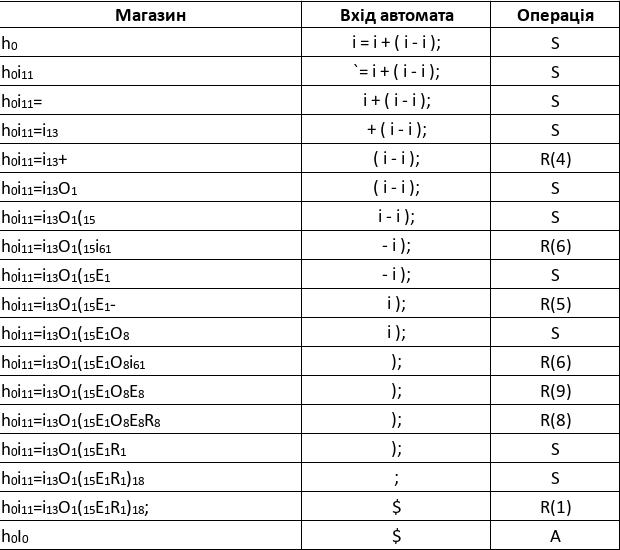
\includegraphics[width=16cm]{reports/formals/assets/pr1.jpeg}
\end{figure}

\clearpage
Перевірка ланцюжка \verb|i = i * ( i + ( i / i ) - i );|
\begin{figure}[h!]
  \centering
  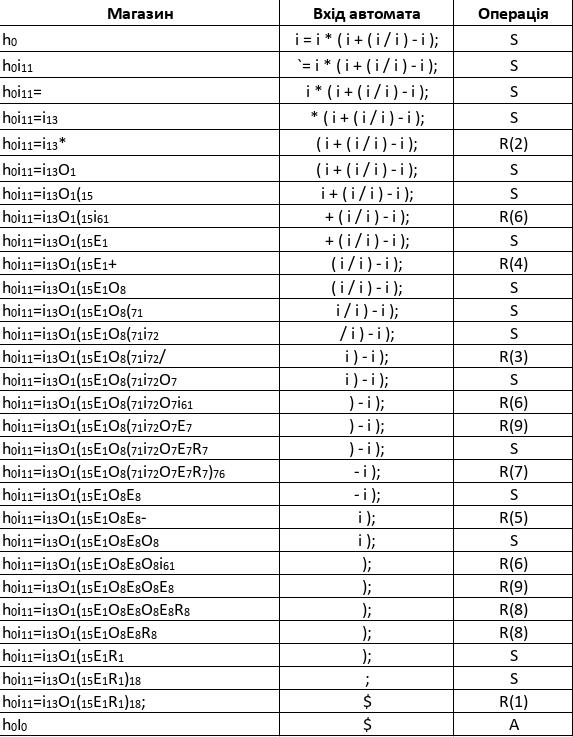
\includegraphics[width=16cm]{reports/formals/assets/pr2.jpeg}
\end{figure}

\clearpage
Перевірка ланцюжка \verb|i = i + ( i + i );|
\begin{figure}[h!]
  \centering
  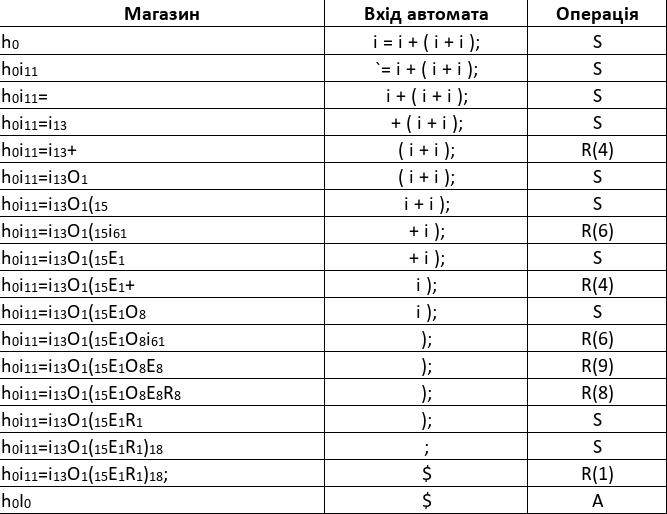
\includegraphics[width=16cm]{reports/formals/assets/pr3.jpeg}
\end{figure}












